\documentclass{../lesson}
\pagestyle{fancy}
\fancyhf{} % 清空页眉页脚
\renewcommand{\headrulewidth}{0.4pt} % 页眉横线
\renewcommand{\footrulewidth}{0pt}   % 页脚横线
\fancyhead[C]{高一物理知识概要}    % 页眉内容（居中）
\fancyfoot[C]{南昌学而思物理组}
\begin{document}
\section{运动的描述}
\concept{机械运动}{\underline{物体}的空间位置随\underline{时间}的变化}
\concept{质点}{有质量的点用于替代物体\\物体的大小、形状和体积对所研究问题的影响可以忽略不计}
\concept{参考系}{处理和使用参考系满足四个性质：\\
\begin{tabular}{cc}
标准性 & 作为参考系的物体被假定是不动的，并且其他的物体的运动与静止都需要相对于这个物体。\\
 任意性 & 参考系的选择是任意的。但是处理问题时一般不能选择物体本身。\\
 统一性 & 研究多个物体需要选同一个参考系。\\
 差异性 & 同一个物体的运动，在不同参考系下一般是不同的。\\
\end{tabular}
}
\notice{高中阶段一般默认地面做参考系，在后面我们会碰到需要更换参考系解决问题的情景。}
\concept{时间}{
    时间间隔，和一段进行的过程相关；时刻，是特定的一瞬间。\\
    未来方便讨论一般需要借助数轴，在上面的认为这就是时间流逝的度量尺，可以人为假定一个时间正方向与原点，也就是零时刻。这个数轴可以命名为时间轴，上面的\underline{点就是时刻，线段代表时间间隔}。
    \begin{tikzpicture}[scale=1.1]
  % 时间轴
  \draw[thick,->] (0,0) -- (7,0) node[right] {时间 $t$/s};
  % 刻度
  \foreach \x in {0,1,2,3,4,5,6}
    \draw (\x,0.12) -- (\x,-0.12);
  % 标签
  \node[below] at (0,0) {0};
  \node[below] at (1,0) {1};
  \node[below] at (2,0) {2};
  \node[below] at (3,0) {3};
  \node[below] at (4,0) {4};
  % 特殊标注
  \draw[thick,red] (1,-0.3) -- (2,-0.3);
  \node[above,red] at (1.5,-0.7) {第2秒};
  \draw[thick,blue] (0,0.3) -- (3,0.3);
  \draw[thick,blue] (0,0) -- (0,0.3);
  \draw[thick,blue] (3,0) -- (3,0.3);
  \node[above,blue] at (1.5,0.35) {前3秒};
  \draw[thick,orange,->] (4,-0.2) -- (4,-0.5);
  \node[below,orange] at (4,-0.5) {第4秒末};
\end{tikzpicture}
}
\concept{位移和路程}{
\begin{minipage}{0.52\textwidth}
    % \vspace{0pt}
\underline{路程} 运动轨迹的长度\\
\underline{位移} 从初位置指向末位置的有向线段\\
图中曲线轨迹为运动轨迹，曲线的长度就是轨迹的长度也是路程。\\
注意里面的位移，位移的变化量和位移很像，但是区别是位移变化量的起点和终点随着每次运动而变化，位移的起点只有一个。
\end{minipage}
\begin{minipage}{0.45\textwidth}
    % \vspace{0pt}
\centering    
\tikzset{every picture/.style={line width=0.75pt}} %set default line width to 0.75pt        
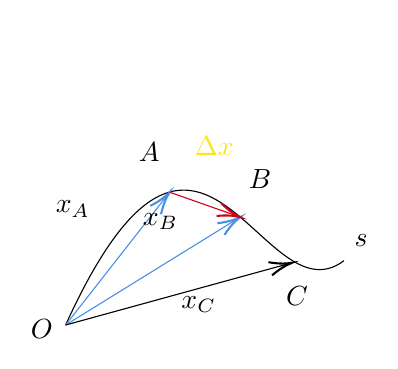
\begin{tikzpicture}[x=0.75pt,y=0.75pt,yscale=-1,xscale=1]
\draw    (80,190) .. controls (145.14,47) and (174.14,189) .. (214.14,159) ;
\draw [color={rgb, 255:red, 74; green, 144; blue, 226 }  ,draw opacity=1 ]   (80,190) -- (128.91,127.57) ;
\draw [shift={(130.14,126)}, rotate = 128.08] [color={rgb, 255:red, 74; green, 144; blue, 226 }  ,draw opacity=1 ][line width=0.75]    (10.93,-3.29) .. controls (6.95,-1.4) and (3.31,-0.3) .. (0,0) .. controls (3.31,0.3) and (6.95,1.4) .. (10.93,3.29)   ;
\draw [color={rgb, 255:red, 74; green, 144; blue, 226 }  ,draw opacity=1 ]   (80,190) -- (162.44,139.05) ;
\draw [shift={(164.14,138)}, rotate = 148.28] [color={rgb, 255:red, 74; green, 144; blue, 226 }  ,draw opacity=1 ][line width=0.75]    (10.93,-3.29) .. controls (6.95,-1.4) and (3.31,-0.3) .. (0,0) .. controls (3.31,0.3) and (6.95,1.4) .. (10.93,3.29)   ;
\draw    (80,190) -- (187.21,160.53) ;
\draw [shift={(189.14,160)}, rotate = 164.63] [color={rgb, 255:red, 0; green, 0; blue, 0 }  ][line width=0.75]    (10.93,-3.29) .. controls (6.95,-1.4) and (3.31,-0.3) .. (0,0) .. controls (3.31,0.3) and (6.95,1.4) .. (10.93,3.29)   ;
\draw [color={rgb, 255:red, 208; green, 2; blue, 27 }  ,draw opacity=1 ]   (130.14,126) -- (162.26,137.33) ;
\draw [shift={(164.14,138)}, rotate = 199.44] [color={rgb, 255:red, 208; green, 2; blue, 27 }  ,draw opacity=1 ][line width=0.75]    (10.93,-3.29) .. controls (6.95,-1.4) and (3.31,-0.3) .. (0,0) .. controls (3.31,0.3) and (6.95,1.4) .. (10.93,3.29)   ;
\draw (114,101) node [anchor=north west][inner sep=0.75pt]    {$A$};
\draw (167,114) node [anchor=north west][inner sep=0.75pt]    {$B$};
\draw (185,170) node [anchor=north west][inner sep=0.75pt]    {$C$};
\draw (141,98) node [anchor=north west][inner sep=0.75pt]  [color={rgb, 255:red, 248; green, 231; blue, 28 }  ,opacity=1 ]  {$\Delta x$};
\draw (74,129) node [anchor=north west][inner sep=0.75pt]    {$x_{A}$};
\draw (116,135) node [anchor=north west][inner sep=0.75pt]    {$x_{B}$};
\draw (134.57,175) node [anchor=north west][inner sep=0.75pt]    {$x_{C}$};
\draw (62,186) node [anchor=north west][inner sep=0.75pt]    {$O$};
\draw (218,145) node [anchor=north west][inner sep=0.75pt]    {$s$};
\end{tikzpicture}
\end{minipage}
}
\notice{后续大家的学习中，位移都是相对于一个固定的初始位置的，末位置是任意时刻的位置，初位置就是运动开始计时的位置。\\
路程是长度，是一个值，不是轨迹。}
\newpage
 \section{运动快慢的描述——速度}
\concept{速度（瞬时速度）}{
    \[v=\lim_{\Delta t\to0}\frac{\Delta x}{\Delta t}\]
    速度是真正的描述物体运动以及快慢的物理量，作为一个矢量，方向代表运动的方向，大小代表那一时刻的运动快慢。}
\concept{平均速度}{
\[\bar{v}=\frac{\Delta x}t\]    
位移除以时间，使用的位移一定是相对于初始位置的，虽然也是矢量，但是其方向不具有任何实际物理意义，大小用来近似表示速度的大小，并且还是一个平均量，只能\underline{反应一段时间内}的快慢水平。}
\concept{瞬时速率}{
\[v_\text{速率}=|v|\]    
瞬时速度的大小，由于速度是矢量，所以瞬时速率是一个标量，并且大于等于0。}
\concept{平均速率}{
\[\bar{v_\text{速率}}=\frac{s}t\]    
平均速率是\underline{路程与时间的比值}，能反应日常生活中的运动快慢，比如长跑中的速率就是平均速率，与运动轨迹相关。}
\concept{x-t图像}{
\begin{minipage}{0.52\textwidth}
    图像中直线斜率代表速度。曲线的切线斜率代表速度。\\
    斜率为负的意味着速度方向和拟定的正方向相反。\\
    图线与时间轴的交点代表物体在坐标为0的位置，图线与纵坐标轴的交点代表物体在初时刻的位置。\\
    图像中任意两个点的\underline{连线斜率}代表两个时刻间的平均速度。
\end{minipage}
\begin{minipage}{0.45\textwidth}
    \centering
\tikzset{every picture/.style={line width=0.75pt}} %set default line width to 0.75pt        
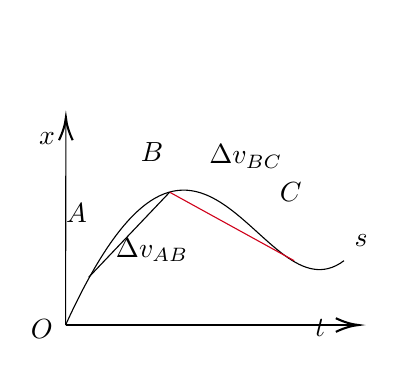
\begin{tikzpicture}[x=0.75pt,y=0.75pt,yscale=-1,xscale=1]
\draw    (80,190) .. controls (145.14,47) and (174.14,189) .. (214.14,159) ;
\draw [color={rgb, 255:red, 208; green, 2; blue, 27 }  ,draw opacity=1 ]   (130.14,126) -- (190.14,159) ;
\draw    (80,190) -- (219.14,190) ;
\draw [shift={(221.14,190)}, rotate = 180] [color={rgb, 255:red, 0; green, 0; blue, 0 }  ][line width=0.75]    (10.93,-3.29) .. controls (6.95,-1.4) and (3.31,-0.3) .. (0,0) .. controls (3.31,0.3) and (6.95,1.4) .. (10.93,3.29)   ;
\draw    (91.14,167) -- (130.14,126) ;
\draw    (80,190) -- (80.14,92) ;
\draw [shift={(80.14,90)}, rotate = 90.08] [color={rgb, 255:red, 0; green, 0; blue, 0 }  ][line width=0.75]    (10.93,-3.29) .. controls (6.95,-1.4) and (3.31,-0.3) .. (0,0) .. controls (3.31,0.3) and (6.95,1.4) .. (10.93,3.29)   ;
\draw (79,130) node [anchor=north west][inner sep=0.75pt]    {$A$};
\draw (115,101) node [anchor=north west][inner sep=0.75pt]    {$B$};
\draw (182,120) node [anchor=north west][inner sep=0.75pt]    {$C$};
\draw (103,147) node [anchor=north west][inner sep=0.75pt]  [color={rgb, 255:red, 0; green, 0; blue, 0 }  ,opacity=1 ]  {$\Delta v_{AB}$};
\draw (62,186) node [anchor=north west][inner sep=0.75pt]    {$O$};
\draw (218,145) node [anchor=north west][inner sep=0.75pt]    {$s$};
\draw (148,102) node [anchor=north west][inner sep=0.75pt]    {$\Delta v_{BC}$};
\draw (66,96) node [anchor=north west][inner sep=0.75pt]    {$x$};
\draw (199,186) node [anchor=north west][inner sep=0.75pt]    {$t$};
\end{tikzpicture}
\end{minipage}
}
\newpage
 \section{描述物体速度变化快慢的物理量——加速度}
\concept{加速度}{
    \[a=\frac{\Delta v}{t}\]
    加速度也是一个矢量，方向代表速度变化的方向，大小代表速度变化的快慢。\\
    加速度与速度变化量的方向相同。下图是速度变化量的求解方法，需要讲速度的起点对齐，然后从初速度的末尾指向末速度的末尾。\\
\tikzset{every picture/.style={line width=0.75pt}} %set default line width to 0.75pt        
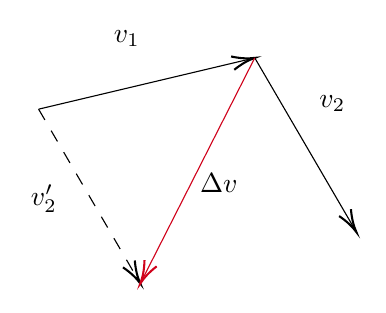
\begin{tikzpicture}[x=0.75pt,y=0.75pt,yscale=-1,xscale=1]
\draw    (322,66) -- (424.2,41.75) ;
\draw [shift={(426.14,41.29)}, rotate = 166.65] [color={rgb, 255:red, 0; green, 0; blue, 0 }  ][line width=0.75]    (10.93,-3.29) .. controls (6.95,-1.4) and (3.31,-0.3) .. (0,0) .. controls (3.31,0.3) and (6.95,1.4) .. (10.93,3.29)   ;
\draw    (426.14,41.29) -- (474.14,123.56) ;
\draw [shift={(475.14,125.29)}, rotate = 239.74] [color={rgb, 255:red, 0; green, 0; blue, 0 }  ][line width=0.75]    (10.93,-3.29) .. controls (6.95,-1.4) and (3.31,-0.3) .. (0,0) .. controls (3.31,0.3) and (6.95,1.4) .. (10.93,3.29)   ;
\draw  [dash pattern={on 4.5pt off 4.5pt}]  (322,66) -- (369.99,148.27) ;
\draw [shift={(371,150)}, rotate = 239.74] [color={rgb, 255:red, 0; green, 0; blue, 0 }  ][line width=0.75]    (10.93,-3.29) .. controls (6.95,-1.4) and (3.31,-0.3) .. (0,0) .. controls (3.31,0.3) and (6.95,1.4) .. (10.93,3.29)   ;
\draw [color={rgb, 255:red, 208; green, 2; blue, 27 }  ,draw opacity=1 ]   (426.14,41.29) -- (371.9,148.22) ;
\draw [shift={(371,150)}, rotate = 296.9] [color={rgb, 255:red, 208; green, 2; blue, 27 }  ,draw opacity=1 ][line width=0.75]    (10.93,-3.29) .. controls (6.95,-1.4) and (3.31,-0.3) .. (0,0) .. controls (3.31,0.3) and (6.95,1.4) .. (10.93,3.29)   ;
\draw (357,27) node [anchor=north west][inner sep=0.75pt]    {$v_{1}$};
\draw (456,58) node [anchor=north west][inner sep=0.75pt]    {$v_{2}$};
\draw (398.57,95.64) node [anchor=north west][inner sep=0.75pt]    {$\Delta v$};
\draw (317,101) node [anchor=north west][inner sep=0.75pt]    {$v_{2} '$};
\end{tikzpicture}\\
    加速度和速度完全没关系。就好像有人问你在哪？你说我刚出门走了200米一样。\\
    和速度类似，不存在加速度与速度变化量成正比这样的说法，只有当a一定时，速度变化量与时间成正比。\\
    由于匀速直线运动，速度不随时间发生变化，所以加速度为0。 \\
    a与v同向，物体做加速运动。\\
a与v反向，减速运动到0，后反向加速运动。\\
a越大，速度变化越快，a越小，速度变化越慢。}
\notice{你知道吗，上面的加速度定义其实是平均加速度的定义式，因为只有在平均物理量，我们才会使用一段时间，并且不要求时间很短。我们的瞬时加速度定义式有两种，一个是和瞬时速度类似的，另一个是利用牛顿第二运动定律（在后期课程大家才会接触）。如下，
\[a=\lim_{t\to0}\frac{\Delta v}{t},a= \frac Fm\]
}
\concept{a-t图像}{这个图像里面，图像与时间轴包围的面积代表这段时间内的速度变化量。\\ 图像在时间轴上方，那么面积认为是正的，否则就是负的，正的面积代表速度变化量为正。 \\ 图像与时间轴的交点意味着此时的加速度为0，一般而言加速度为0，左右如果图像分布在时间轴的上下两侧，物体运动减速，注意仅仅是减速。}
\concept{匀变速直线运动}{为加速度恒定的直线运动，大小和方向都不变。所以有下面的公式成立：
\[a=\frac{v-v_0}{t}=\frac{\Delta v}{t}\]
}
\newpage
\section{匀变速直线运动规律}
\concept{v-t图像怎么用？}{
\begin{minipage}{0.52\textwidth}
    匀变速直线运动的图像在v-t图像中，表达式为$v=at+v_0$，也就是斜率是a，截距是$v_0$的直线。\\ v-t图像中（切线）斜率代表加速度。\\ 与t轴的交点附近，如果左右图线穿过t轴，那么物体将会在$v=0$也就是交点处反向运动。\\ 在一段时间内，图像与t轴包围的面积代表这段时间内的位移。\\ 注意一下，如果面积在t轴上方，那么面积认为是正的，否则就是负的，正的面积代表位移为正。\\
\end{minipage}
\hfill    
\begin{minipage}
{0.45\textwidth}
    \centering
    \begin{tikzpicture}[scale=1.2]
  % 坐标轴
  \draw[->] (0,0) -- (5,0) node[right] {$t$};
  \draw[->] (0,-2) -- (0,2) node[above] {$v$};
  % 两根竖线
  \draw[dashed] (1,-1.2) -- (1,1.2);
  \draw[dashed] (4.5,-1.5) -- (4.5,1.5);
  % 曲线
  \draw[thick,domain=1:4.5,smooth,variable=\x] 
    plot ({\x},{1.5-1.2*(\x-2)^2/2});
  % 上方面积填充（东北方向平行线）
  \begin{scope}
    \clip (1,0) -- plot[domain=1:3.6,smooth] ({\x},{1.5-1.2*(\x-2)^2/2}) -- (3.6,0) -- cycle;
    \fill[pattern=north east lines,pattern color=blue!60] (1,0) -- plot[domain=1:3.6,smooth] ({\x},{1.5-1.2*(\x-2)^2/2}) -- (3.6,0) -- cycle;
  \end{scope}
  % 下方面积填充（西北方向平行线）
  \begin{scope}
    \clip (3.6,0) -- plot[domain=3.6:4.5,smooth] ({\x},{1.5-1.2*(\x-2)^2/2}) -- (4.5,0) -- cycle;
    \fill[pattern=north west lines,pattern color=orange!70!black] (3.6,0) -- plot[domain=3.6:4.5,smooth] ({\x},{1.5-1.2*(\x-2)^2/2}) -- (4.5,0) -- cycle;
  \end{scope}
  % 曲线再画一遍盖住填充边界
  \draw[thick,domain=1:4.5,smooth,variable=\x] 
    plot ({\x},{1.5-1.2*(\x-2)^2/2});
  % 标注
  \node[below] at (1,0) {$t_1$};
  \node[below] at (4.5,0) {$t_3$};
  \node[below] at (3.6,0) {$t_2$};
\end{tikzpicture}
\end{minipage}
}
\concept{匀变速直线运动x-t公式}{
\begin{minipage}{0.5\textwidth}\[x=v_0t+\frac12at^2+x_0\]
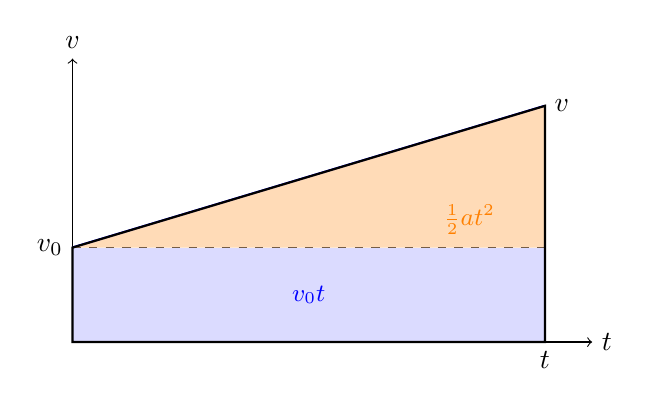
\begin{tikzpicture}[scale=1.2]
  % 坐标轴
  \draw[->] (0,0) -- (5.5,0) node[right] {$t$};
  \draw[->] (0,0) -- (0,3) node[above] {$v$};
  % 斜率为a的直线
  \draw[thick,blue] (0,1) -- (5,2.5);
  % 辅助线
  \draw[dashed] (0,1) -- (5,1);
  \draw[dashed] (5,0) -- (5,2.5);
  % 矩形
  \fill[blue!20,opacity=0.7] (0,0) -- (5,0) -- (5,1) -- (0,1) -- cycle;
  % 三角形
  \fill[orange!40,opacity=0.7] (0,1) -- (5,1) -- (5,2.5) -- cycle;
  % 边框
  \draw[thick] (0,1) -- (5,2.5) -- (5,0) -- (0,0) -- cycle;
  % 标注
  \node[left] at (0,1) {$v_0$};
  \node[right] at (5,2.5) {$v$};
  \node[below] at (5,0) {$t$};
  % 公式标注
  \node at (2.5,0.5) {\small $\textcolor{blue}{v_0 t}$};
  \node at (4.2,1.3) {\small $\textcolor{orange}{\frac{1}{2}at^2}$};
\end{tikzpicture}
\end{minipage}
\hfill
\begin{minipage}{0.5\textwidth}\[x=vt-\frac12at^2+x_0\]
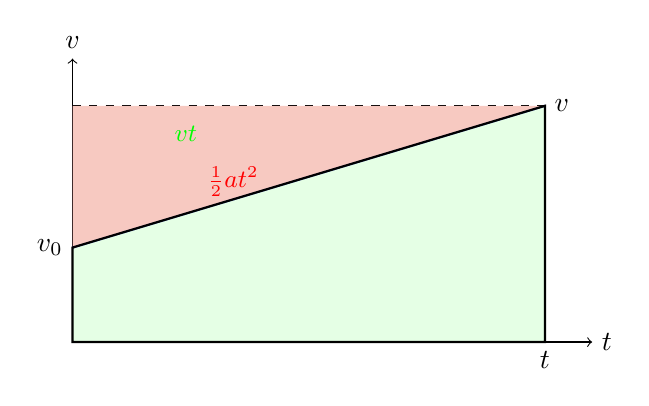
\begin{tikzpicture}[scale=1.2]
  % 坐标轴
  \draw[->] (0,0) -- (5.5,0) node[right] {$t$};
  \draw[->] (0,0) -- (0,3) node[above] {$v$};
  % 斜率为a的直线
  \draw[thick,blue] (0,1) -- (5,2.5);
  % 辅助线
  \draw[dashed] (0,2.5) -- (5,2.5);
  \draw[dashed] (5,0) -- (5,2.5);
  % 大矩形
  \fill[green!20,opacity=0.5] (0,0) -- (5,0) -- (5,2.5) -- (0,2.5) -- cycle;
  % 补的三角形
  \fill[red!30,opacity=0.7] (0,1) -- (0,2.5) -- (5,2.5) -- cycle;
  % 边框
  \draw[thick] (0,1) -- (5,2.5) -- (5,0) -- (0,0) -- cycle;
  % 标注
  \node[left] at (0,1) {$v_0$};
  \node[right] at (5,2.5) {$v$};
  \node[below] at (5,0) {$t$};
  % 公式标注
  \node at (1.2,2.2) {\small $\textcolor{green}{vt}$};
  \node at (1.7,1.7) {\small $\textcolor{red}{\frac{1}{2}at^2}$};
\end{tikzpicture}
\end{minipage}
\begin{minipage}
{0.5\textwidth}
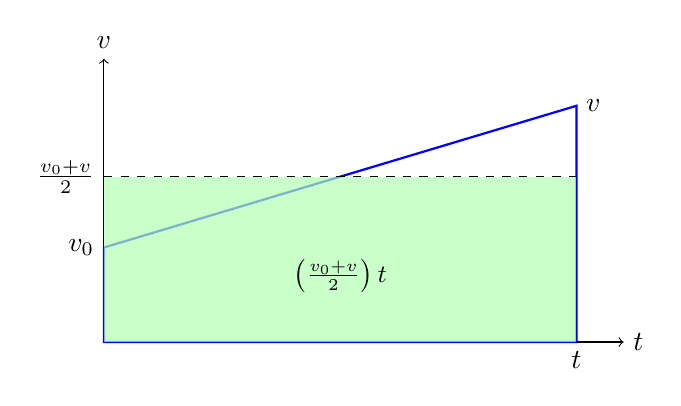
\begin{tikzpicture}[scale=1.2]
  % 坐标轴
  \draw[->] (0,0) -- (5.5,0) node[right] {$t$};
  \draw[->] (0,0) -- (0,3) node[above] {$v$};
  % 梯形顶点
  \coordinate (A) at (0,1);
  \coordinate (B) at (5,2.5);
  \coordinate (C) at (5,0);
  \coordinate (D) at (0,0);
  % 梯形
  \draw[thick,blue] (A) -- (B) -- (C) -- (D) -- cycle;
  % 辅助线：中间矩形
  \coordinate (M1) at (0,1.75);
  \coordinate (M2) at (5,1.75);
  \draw[dashed] (M1) -- (M2);
  % 填充中间矩形
  \fill[green!30,opacity=0.7] (0,0) -- (5,0) -- (5,1.75) -- (0,1.75) -- cycle;
  % 标注
  \node[left] at (A) {$v_0$};
  \node[right] at (B) {$v$};
  \node[below] at (5,0) {$t$};
  \node[left] at (M1) {$\frac{v_0+v}{2}$};
  % 公式标注
  \node at (2.5,0.7) {\small $\left(\frac{v_0+v}{2}\right)t$};
\end{tikzpicture}
\end{minipage}
\hfill
\begin{minipage}
{0.5\textwidth}\[x=\frac{v_0+v}2t=\bar v t\]
\end{minipage}
}
\notice{
    你会注意到，上面是x关于t的一元二次方程，注意加速度里面有$\frac12$。\\
    上面两个公式，是通过两个不同的角度观察一元二次方程，从初始分析，和从结束逆推。
}
\concept{匀变速直线运动x-v公式}{
    \[v^2=v_0^2+2ax\]
}
\newpage
\section{自由落体运动相关}
\concept{自由落体运动}{就是特殊的匀加速直线运动，初速度为0，加速度为重力加速度，方向竖直向下。下面是基本公式：
\[x=\frac12gt^2\]
\[v=\sqrt{2gx}\]
\[t=\sqrt{\frac{2x}{g}}\]
}
\notice{你知道吗？自由落体类似的匀变速直线运动有着非常有趣的二级结论：
\begin{itemize}
  \item 相同时间间隔每段位移之比是1:3:5
  \item 相同位移间隔每段时间之比是1:$\sqrt2-1$:$\sqrt3-\sqrt2$
\end{itemize}}
\concept{竖直上抛运动}{就是特殊的匀减速直线运动，并且可能包含返回。\\初速度不等于0，加速度为重力加速度，方向竖直向下。公式只需要把匀变速直线运动的加速度替换即可，此处省略。\\
比较有趣的事情是，匀变速直线运动中，所有的返回加速过程与减速过程是关于返回点对称的，也就是说物体减速经过某个点，之后再返回过程中将会是速度大小相同，但是方向相反的。}
\notice{
  运动学的多解，可以是位移大小相同，方向未知，也可以是速度大小相同，方向未知。甚至可以是两者同时存在。使得我们会有两解、甚至三解的情况。
}
\newpage
 \section{运动学综合提升}
\concept{5个基本公式}{
\[v=v_0+at\]
\[x=v_0t+\frac12at^2+x_0\]
\[x=vt-\frac12at^2+x_0\]
\[x=\bar vt=\frac{v_0+v_t}{2}t\]
\[v_t^2-v_0^2=2ax\]
在诸多公式里面我最喜欢，也最擅长使用两个。\[x=\frac{\bar v}{t}=\frac{v_0+v_t}{2t}\]这个公式也有一个文字描述，中间时刻的瞬时速度等于平均速度。只要发现题目给了一段位移并且有这段位移所花费的时间，那么这个公式是首选。然后计算出中间时刻的速度。\[v^2-v_0^2=2ax\]这个公式由于缺少时间，所以特征非常明显，一般情况下，如果题目缺少很多时间变量，那么可以考虑用这个公式。}
\concept{x-t图像理解}{
\begin{itemize}
  \item \emph{（切线）斜率代表速度}，正斜率表示正向运动，负斜率表示反向运动。
  \item \emph{在图像的转折点或者是v=0，并且左右斜率正负不相同的地方}是运动反向点。
  \item 匀速直线运动是任意一条水平线。
  \item 匀变速直线运动是一条一元二次函数图像。
\end{itemize}
}
\concept{v-t图像理解}{
\begin{itemize}
  \item \emph{（切线）斜率代表加速度}，正斜率表示加速运动，负斜率表示减速运动。
  \item \emph{与t轴的交点，左右如果正负不同}，那么这就是运动反向点。
  \item 匀速直线运动是一条$v=0$的水平线。
  \item 匀变速直线运动是一条倾斜的直线。
  \item 与t轴围成的面积代表位移，面积在t轴上方表示正向位移，面积在t轴下方表示反向位移。
  \item \underline{v-t图像没有位置信息，只有位移，所以无法直接确定多物体的相对位置关系。}
\end{itemize}
}
\newpage
\concept{拓展公式}{
\[v_{\frac12t}=\bar v=\frac{v_0+v_t}{2}\]
\[v_{\frac12x}=\sqrt{\frac{v_0^2+v_t^2}{2}}\]
一般情况下，相等时间间隔$T$，第M段与第N段的位移之差为
\[\Delta x_{M,N}=(M-N)aT^2\]
在初速度为0时有两个特殊结论：下面是相等时间间隔，
\[\text{累计速度比}=1:2:\cdots:n\]
\[\text{累计位移比}=1:2^2:\cdots:n^2\]
\[\text{每段位移比}=1:3:\cdots:2n-1\]
下面是相等位移间隔，
\[\text{每段时间比}=1:\sqrt{2}-1:\cdots:\sqrt{n}-\sqrt{n-1}\]
\[\text{累计速度比}=1:\sqrt{2}:\cdots:\sqrt{n}\]
\[\text{累计时间比}=1:\sqrt{2}:\cdots:\sqrt{n}\]
(拓展公式用于课外，课堂上我们会在秋季课正式讲解。累计时间位移等，这只是一种标记手段，意思是累计多段)\\
\begin{minipage}{0.48\textwidth}
\centering
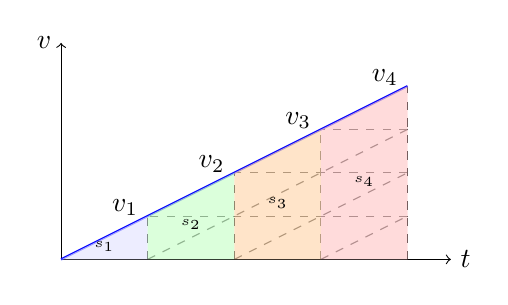
\begin{tikzpicture}[scale=1.1]
  % 坐标轴
  \draw[->] (0,0) -- (0,2.5) node[left] {$v$};
  \draw[->] (0,0) -- (4.5,0) node[right] {$t$};
  % 等时间间隔
  \foreach \i in {1,2,3,4}
    \draw[dashed] (\i,0) -- (\i,\i*0.5);
  \foreach \i in {1,2,3} 
    \draw[dashed] (4,\i*0.5) -- (\i,\i*0.5);
  \foreach \i in {1,2,3}
    \draw[dashed] (\i,0) -- (4,2-\i*0.5);
  % 匀加速直线
  \draw[thick,blue] (0,0) -- (4,2);
  % 速度标记
  \foreach \i/\v in {0/1,1/2,2/3,3/4}
    \node[left] at (\i+1,\i*0.5+0.6) {$v_{\the\numexpr\i+1}$};
  % % 速度比箭头
  % \foreach \i in {0,1,2}
  %   \draw[<->,red] (\i,0.5+\i*0.833) -- (\i+1,0.5+(\i+1)*0.833);
  % 时间标记
  % \foreach \i in {1,2,3}
  %   \node[below] at (\i,0) {$t_{\i}$};
  % 位移阴影
  \foreach \i/\col in {0/blue!10, 1/green!20, 2/orange!30, 3/red!20} {
    \fill[\col,opacity=0.7] (\i,0) -- (\i+1,0) -- (\i+1,\i*0.5+0.5) -- (\i,\i*0.5);
    \node at (\i+0.5,\i*0.25+0.15) {\tiny $s_{\the\numexpr\i+1}$};
  }
\end{tikzpicture}
\end{minipage}
\hfill
\begin{minipage}{0.48\textwidth}
\centering
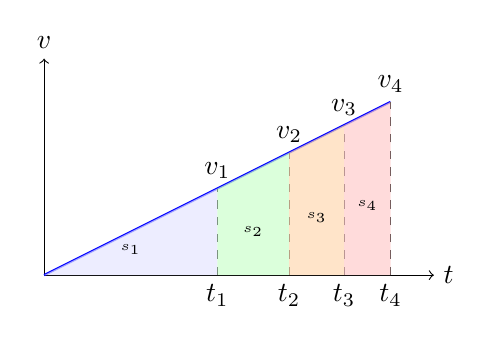
\begin{tikzpicture}[scale=1.1]
  % 坐标轴
  \draw[->] (0,0) -- (0,2.5) node[above] {$v$};
  \draw[->] (0,0) -- (4.5,0) node[right] {$t$};
  % 匀加速直线
  \draw[thick,blue] (0,0) -- (4,2);
  % 等位移间隔
  \foreach \i in {1,2,3,4}
    \draw[dashed] ({2*sqrt(\i)},0) -- ({2*sqrt(\i)},{sqrt(\i)});
  % 时间标记
  \node[below] at (2,0) {$t_1$};
  \node[below] at ({2*sqrt(2)},0) {$t_2$};
  \node[below] at ({2*sqrt(3)},0) {$t_3$};
  \node[below] at ({2*sqrt(4)},0) {$t_4$};
  % % 位移阴影
  \foreach \i/\col in {1/blue!10, 2/green!20, 3/orange!30, 4/red!20} {
    \fill[\col,opacity=0.7] ({2*sqrt(\i-1)},0) -- ({2*sqrt(\i)},0) -- ({2*sqrt(\i)},{sqrt(\i)}) -- ({2*sqrt(\i-1)},{sqrt(\i-1)});
    \node at ({(sqrt(\i)+sqrt(\i-1))},{sqrt(\i)*0.5-0.2}) {\tiny $s_{\the\numexpr\i}$};
  }
  \foreach \i in {1,2,3,4}
    \node[above] at ({2*sqrt(\i)},{sqrt(\i)}) {$v_{\the\numexpr\i}$};
\end{tikzpicture}
\end{minipage}
}
\newpage
 \section{相互作用力}
\equations{
  G=mg
}
\concept{重力}{
  方向常考，竖直向下，不是垂直向下，可以是垂直水平面向下。\\
  重力不会因物体的运动而改变，只有两个因素，质量和重力加速度。重力加速度本身也只和物体所在位置和海拔高度。\\
  重力的产生原因：万有引力+圆周运动。\\
  重力是最简单的力，所以分析的时候一般先分析重力。
}
\concept{弹力}{有形变，想要恢复形变的力叫弹力，弹力的方向：
一般情况下，有明确的接触面的弹力，方向沿着接触面法线方向。（就是垂直于接触面指向受力物体）\\
但是接触面很多种，
\begin{itemize}
  \item 面面接触：接触面法线方向。
  \item 点面接触：面的法线方向。
  \item 点点接触：分为有无圆面（因为圆一般和其他物体接触只有一个接触点）有圆面一定是圆的切面法线方向指向受力物体；否则就是两个点的重心的连线方向。
\end{itemize}
绳子提供的弹力只能沿绳方向，只能提供拉力，\\
杆子可以像绳子一样提供拉力或支持力，但是杆子的弹力可以是沿杆方向也可以是任意方向，取决于杆子的一端是否固定。举几个例子\\ \newline
\begin{minipage}{0.52\textwidth}
    图中，$N_1$来源于圆形物体的形变，$N_2$来源于杆子的形变，$N_1$这种由圆形物体形变产生的弹力方向一定是沿半径指向圆心。$N_2$由杆子形变产生，方向必然沿杆子和圆形物体的接触面的法线方向。\\
    另一个角度思考，在底部的地方，是点和圆面接触，那么方向必然是圆面的法线方向。在$N_2$位置，是点与杆面的接触，所以必然是沿杆子所在面的法线方向。
\end{minipage}
\begin{minipage}{0.45\textwidth}
\centering
\tikzset{every picture/.style={line width=0.75pt}} 
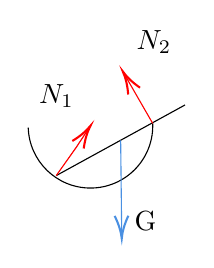
\begin{tikzpicture}[x=0.75pt,y=0.75pt,yscale=-1,xscale=1]
\draw  [draw opacity=0] (109.98,68.85) .. controls (109.99,69.23) and (110,69.61) .. (110,70) .. controls (110,86.57) and (96.57,100) .. (80,100) .. controls (63.74,100) and (50.5,87.06) .. (50.01,70.91) -- (80,70) -- cycle ; \draw   (109.98,68.85) .. controls (109.99,69.23) and (110,69.61) .. (110,70) .. controls (110,86.57) and (96.57,100) .. (80,100) .. controls (63.74,100) and (50.5,87.06) .. (50.01,70.91) ;  
\draw    (63.5,94) -- (125.57,59.96) ;
\draw [color={rgb, 255:red, 255; green, 0; blue, 0 }  ,draw opacity=1 ][fill={rgb, 255:red, 255; green, 0; blue, 0 }  ,fill opacity=1 ]   (63.5,94) -- (73.14,80.43) -- (78.9,71.67) ;
\draw [shift={(80,70)}, rotate = 123.33] [color={rgb, 255:red, 255; green, 0; blue, 0 }  ,draw opacity=1 ][line width=0.75]    (10.93,-3.29) .. controls (6.95,-1.4) and (3.31,-0.3) .. (0,0) .. controls (3.31,0.3) and (6.95,1.4) .. (10.93,3.29)   ;
\draw [color={rgb, 255:red, 255; green, 0; blue, 0 }  ,draw opacity=1 ]   (109.98,68.85) -- (96.57,45.55) ;
\draw [shift={(95.57,43.82)}, rotate = 60.07] [color={rgb, 255:red, 255; green, 0; blue, 0 }  ,draw opacity=1 ][line width=0.75]    (10.93,-3.29) .. controls (6.95,-1.4) and (3.31,-0.3) .. (0,0) .. controls (3.31,0.3) and (6.95,1.4) .. (10.93,3.29)   ;
\draw [color={rgb, 255:red, 74; green, 144; blue, 226 }  ,draw opacity=1 ]   (94.54,76.98) -- (95.05,122.32) ;
\draw [shift={(95.07,124.32)}, rotate = 269.35] [color={rgb, 255:red, 74; green, 144; blue, 226 }  ,draw opacity=1 ][line width=0.75]    (10.93,-3.29) .. controls (6.95,-1.4) and (3.31,-0.3) .. (0,0) .. controls (3.31,0.3) and (6.95,1.4) .. (10.93,3.29)   ;
\draw (100,110) node [anchor=north west][inner sep=0.75pt]   [align=left] {G};
\draw (101,23) node [anchor=north west][inner sep=0.75pt]   [align=left] {$\displaystyle N_{2}$};
\draw (54,49) node [anchor=north west][inner sep=0.75pt]   [align=left] {$\displaystyle N_{1}$};
\end{tikzpicture}
\end{minipage}
\begin{minipage}{0.45\textwidth}
    \centering
    \tikzset{every picture/.style={line width=0.75pt}} 
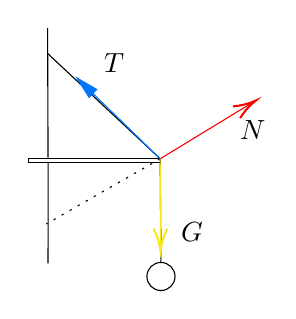
\begin{tikzpicture}[x=0.75pt,y=0.75pt,yscale=-1,xscale=1]
\draw    (269.9,67.1) -- (270.12,129.47) ;
\draw    (269.9,79.24) -- (324.14,130) ;
\draw   (260.57,130) -- (324.14,130) -- (324.14,131.9) -- (260.57,131.9) -- cycle ;
\draw    (270.12,131.61) -- (270.16,140.58) -- (270.11,180.34) ;
\draw    (324.14,130) -- (324.51,179.94) ;
\draw   (317.75,186.71) .. controls (317.75,182.97) and (320.78,179.94) .. (324.51,179.94) .. controls (328.25,179.94) and (331.28,182.97) .. (331.28,186.71) .. controls (331.28,190.45) and (328.25,193.48) .. (324.51,193.48) .. controls (320.78,193.48) and (317.75,190.45) .. (317.75,186.71) -- cycle ;
\draw [color={rgb, 255:red, 255; green, 0; blue, 0 }  ,draw opacity=1 ]   (324.14,130) -- (368.58,102.93) ;
\draw [shift={(370.29,101.89)}, rotate = 148.65] [color={rgb, 255:red, 255; green, 0; blue, 0 }  ,draw opacity=1 ][line width=0.75]    (10.93,-3.29) .. controls (6.95,-1.4) and (3.31,-0.3) .. (0,0) .. controls (3.31,0.3) and (6.95,1.4) .. (10.93,3.29)   ;
\draw  [dash pattern={on 0.84pt off 2.51pt}]  (324.14,130) -- (269.29,161.39) ;
\draw [color={rgb, 255:red, 0; green, 117; blue, 255 }  ,draw opacity=1 ]   (324.14,130) -- (284.72,91.71) ;
\draw [shift={(283.29,90.32)}, rotate = 44.16] [fill={rgb, 255:red, 0; green, 117; blue, 255 }  ,fill opacity=1 ][line width=0.08]  [draw opacity=0] (12,-3) -- (0,0) -- (12,3) -- cycle    ;
\draw [color={rgb, 255:red, 248; green, 231; blue, 28 }  ,draw opacity=1 ]   (324.14,130) -- (324.28,172.54) ;
\draw [shift={(324.29,174.54)}, rotate = 269.82] [color={rgb, 255:red, 248; green, 231; blue, 28 }  ,draw opacity=1 ][line width=0.75]    (10.93,-3.29) .. controls (6.95,-1.4) and (3.31,-0.3) .. (0,0) .. controls (3.31,0.3) and (6.95,1.4) .. (10.93,3.29)   ;
\draw (332.93,159.5) node [anchor=north west][inner sep=0.75pt]    {$G$};
\draw (295.93,78) node [anchor=north west][inner sep=0.75pt]    {$T$};
\draw (361.43,110.5) node [anchor=north west][inner sep=0.75pt]    {$N$};
\end{tikzpicture}
\end{minipage}
\begin{minipage}{0.52\textwidth}
    杆子插在墙壁里面，或者是题目说了固定的杆子，那么杆子所提供的弹力方向将不会沿着杆子，方向是未知且任意可能的。
\end{minipage}
\begin{minipage}{0.52\textwidth}
弹簧作为特殊的弹力产生物体，可以像绳子一样产生拉力，也可以像杆子一样提供支持力。
\end{minipage}
\begin{minipage}{0.45\textwidth}
\centering
\tikzset{every picture/.style={line width=0.75pt}} 
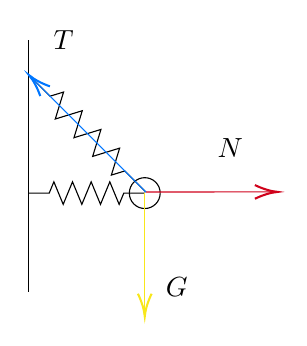
\begin{tikzpicture}[x=0.75pt,y=0.75pt,yscale=-1,xscale=1]
\draw   (450,123.43) -- (460.11,123.43) -- (462.35,118) -- (466.84,128.86) -- (471.33,118) -- (475.83,128.86) -- (480.32,118) -- (484.81,128.86) -- (489.3,118) -- (493.79,128.86) -- (496.04,123.43) -- (506.14,123.43) ;
\draw   (450.39,66.61) -- (460.52,76.74) -- (467.02,74.75) -- (463.03,87.74) -- (476.03,83.75) -- (472.03,96.75) -- (485.03,92.76) -- (481.04,105.75) -- (494.04,101.76) -- (490.05,114.76) -- (496.54,112.76) -- (506.68,122.9) ;
\draw    (450.14,49.86) -- (450.14,170.86) ;
\draw   (498.71,123.43) .. controls (498.71,119.33) and (502.04,116) .. (506.14,116) .. controls (510.25,116) and (513.57,119.33) .. (513.57,123.43) .. controls (513.57,127.53) and (510.25,130.86) .. (506.14,130.86) .. controls (502.04,130.86) and (498.71,127.53) .. (498.71,123.43) -- cycle ;
\draw [color={rgb, 255:red, 248; green, 231; blue, 28 }  ,draw opacity=1 ]   (506.14,123.43) -- (506.14,180.86) ;
\draw [shift={(506.14,182.86)}, rotate = 270] [color={rgb, 255:red, 248; green, 231; blue, 28 }  ,draw opacity=1 ][line width=0.75]    (10.93,-3.29) .. controls (6.95,-1.4) and (3.31,-0.3) .. (0,0) .. controls (3.31,0.3) and (6.95,1.4) .. (10.93,3.29)   ;
\draw [color={rgb, 255:red, 208; green, 2; blue, 27 }  ,draw opacity=1 ]   (506.68,122.9) -- (568.14,122.86) ;
\draw [shift={(570.14,122.86)}, rotate = 179.97] [color={rgb, 255:red, 208; green, 2; blue, 27 }  ,draw opacity=1 ][line width=0.75]    (10.93,-3.29) .. controls (6.95,-1.4) and (3.31,-0.3) .. (0,0) .. controls (3.31,0.3) and (6.95,1.4) .. (10.93,3.29)   ;
\draw [color={rgb, 255:red, 0; green, 118; blue, 255 }  ,draw opacity=1 ]   (506.68,122.9) -- (451.8,68.02) ;
\draw [shift={(450.39,66.61)}, rotate = 45] [color={rgb, 255:red, 0; green, 118; blue, 255 }  ,draw opacity=1 ][line width=0.75]    (10.93,-3.29) .. controls (6.95,-1.4) and (3.31,-0.3) .. (0,0) .. controls (3.31,0.3) and (6.95,1.4) .. (10.93,3.29)   ;
\draw (515,163) node [anchor=north west][inner sep=0.75pt]    {$G$};
\draw (540,96) node [anchor=north west][inner sep=0.75pt]    {$N$};
\draw (461,44) node [anchor=north west][inner sep=0.75pt]    {$T$};
\end{tikzpicture}
\end{minipage}
}
\newpage
\equations{
  F=kx
}
\concept{弹簧弹力}{
\begin{minipage}{0.9\textwidth}
\centering
\begin{tikzpicture}[scale=1.2]
  % 竖直位置
  \def\yA{2.5}
  \def\yB{1.2}
  \def\yC{0}
  % 弹簧长度
  \def\L{2.5}
  \def\stretch{1.0}
  \def\compress{1.0}
  % 左端对齐的x坐标
  \def\xL{0.5}
  % 右端x坐标
  \def\xA{\xL+\L}
  \def\xB{\xL+\L+\stretch}
  \def\xC{\xL+\L-\compress}
  % 原长弹簧
  \draw[thick,decorate,decoration={coil,aspect=0.5,segment length=3mm,amplitude=2mm}] (\xL,\yA) -- (\xA,\yA);
  \filldraw[gray] (\xL,\yA) circle (0.09);
  \filldraw[gray] (\xA,\yA) circle (0.09);
  \node[above] at ({(\xL+\xA)/2},\yA+0.18) {\small 原长 $l_0$};
  % 拉伸弹簧
  \draw[thick,decorate,decoration={coil,aspect=0.5,segment length=3mm,amplitude=2mm}] (\xL,\yB) -- (\xB,\yB);
  \filldraw[gray] (\xL,\yB) circle (0.09);
  \filldraw[gray] (\xB,\yB) circle (0.09);
  % 拉力箭头
  \draw[->,red,thick] (\xB,\yB) -- ++(0.7,0) node[right] {\small $F_\text{拉}$};
  \node[above] at ({(\xL+\xB)/2},\yB+0.18) {\small 拉伸 $l_0+\Delta l$};
  % 压缩弹簧
  \draw[thick,decorate,decoration={coil,aspect=0.5,segment length=3mm,amplitude=2mm}] (\xL,\yC) -- (\xC,\yC);
  \filldraw[gray] (\xL,\yC) circle (0.09);
  \filldraw[gray] (\xC,\yC) circle (0.09);
  % 压力箭头
  \draw[<-,blue,thick] (\xC,\yC) -- ++ (0.7,0) node[right] {\small $F_\text{压}$};
  \node[above] at ({(\xL+\xC)/2},\yC+0.18) {\small 压缩 $l_0-\Delta l$};
  % 末端比较连线
  \draw[thick,gray!60!black,dashed] (\xA,\yA) -- (\xA,\yC);
  \draw[thick,gray!60!black,dashed] (\xB,\yA) -- (\xB,\yC);
  \draw[thick,gray!60!black,dashed] (\xC,\yA) -- (\xC,\yC);
\end{tikzpicture}
\end{minipage}\\
	发生弹性形变时，弹簧的弹力与弹簧的形变量成正比。比值叫做劲度系数。劲度系数只与弹簧本身有关，和弹簧的圈数呈正比，和材料有关，与直径有关，等等。\\
  \[x=|l-l_0|\]
  \begin{itemize}
    \item 上面的形变量的计算公式，注意里面的$l_0$指弹簧不受力时长度，叫做原长。绝对值即弹簧处于压缩状态，弹簧长度将会小于原长。
    \item 弹簧处于压缩状态，弹力向两侧，弹簧处于拉伸状态，弹力向内。
    \item 弹簧弹力等于任何一端的受力，
    \item 弹簧两端的受力一定大小相等，方向相反，不管处于何种运动状态下。
    \item 弹力只和形变量有关，也就意味着，弹力不会直接因为物体运动状态改变而改变，除非弹簧形变量变化。
  \end{itemize}
  \begin{minipage}{0.48\textwidth}
\centering
\begin{tikzpicture}[scale=1.1]
  % 弹簧
  \draw[thick,decorate,decoration={coil,aspect=0.5,segment length=4mm,amplitude=2mm}] (0,0) -- (3,0);
  % 左端固定
  \filldraw[gray] (0,0) circle (0.12);
  % 右端小球
  \filldraw[gray] (3,0) circle (0.18);
  % 受力箭头
  \draw[->,blue,thick] (3,0) -- (2.2,0) node[left] {$F_\text{弹}$};
  \draw[->,blue,thick] (0,0) -- (0.8,0) node[right] {$F_\text{弹}$};
  % 文字
  \node[below] at (1.5,-0.3) {\small 拉伸：$F_\text{弹}$ 向内};
\end{tikzpicture}
\end{minipage}
\hfill
\begin{minipage}{0.48\textwidth}
\centering
\begin{tikzpicture}[scale=1.1]
  % 弹簧
  \draw[thick,decorate,decoration={coil,aspect=0.5,segment length=2.5mm,amplitude=2mm}] (0,0) -- (1.5,0);
  % 左端固定
  \filldraw[gray] (0,0) circle (0.12);
  % 右端小球
  \filldraw[gray] (1.5,0) circle (0.18);
  % 受力箭头
  \draw[->,blue,thick] (0,0) -- (-0.8,0) node[left] {$F_\text{弹}$};
  \draw[->,blue,thick] (1.5,0) -- (2.3,0) node[right] {$F_\text{弹}$};
  % 文字
  \node[below] at (0.75,-0.3) {\small 压缩：$F_\text{弹}$ 向外};
\end{tikzpicture}
\end{minipage}
}
\concept{弹簧的劲度系数}{
  并联弹簧劲度系数 $k_\text{并} = k_1 + k_2 + \cdots + k_n$\\
  串联弹簧劲度系数 $\frac1{k_\text{串}} = \frac{1}{k_1} + \frac{1}{k_2} + \cdots + \frac{1}{k_n}$\\
  当只有两根弹簧时，串联和并联的关系可以简化为：
  \[
  k_\text{并} = k_1 + k_2, \quad k_\text{串} = \frac{k_1 k_2}{k_1 + k_2}
  \]
  由此可以知道，\underline{把一根弹簧进行分割时，如果分成两段，分割后两段的劲度系数是原来的两倍！}\\
  分成$n$段，分割后每段的劲度系数是原来的$n$倍。\\
  之后并联这些分段，整体的劲度系数达到了惊人的$n^2$倍！\\
}
\newpage
\section{摩擦力}
\equations{
  f_{\text{滑}} = \mu N\quad f_{\text{静}} \leqslant  f_{\text{最大静摩擦力}}}
\concept{摩擦力}{
\begin{itemize}
  \item \textbf{摩擦力的定义}：摩擦力是两个\emph{相互接触}并有\emph{相对运动趋势或相对运动}的物体之间，在接触面上产生的阻碍相对运动的力。\\
  摩擦力的方向总是与相对运动方向相反，或与相对运动趋势方向相反。
  \item \textbf{摩擦力的分类}：
    \begin{itemize}
      \item \emph{静摩擦力}：当物体间没有发生相对滑动，但有相对滑动趋势时，接触面之间产生的阻碍相对运动趋势的力叫静摩擦力。静摩擦力的大小随外力变化而变化，其最大值称为最大静摩擦力。
      \item \emph{滑动摩擦力}：当物体间发生相对滑动时，接触面之间产生的阻碍相对滑动的力叫滑动摩擦力。滑动摩擦力的大小通常为恒定值。
      \item \emph{滚动摩擦力}：当物体在另一物体表面滚动时，产生的阻碍滚动的力叫滚动摩擦力。滚动摩擦力远小于滑动摩擦力。
    \end{itemize}
  \item \textbf{摩擦力的产生条件}：
    \begin{itemize}
      \item 必须有两个物体相互接触，
      \item 相互产生弹力，
      \item 并且接触面具有粗糙性（微观不平），
      \item 且有相对运动或相对运动趋势。
    \end{itemize}
  \item \textbf{摩擦力的方向}：总是与物体相对运动方向或相对运动趋势方向相反。
  \item \textbf{摩擦力的计算公式}：
    \begin{itemize}
      \item 最大静摩擦力与正压力成正比，而静摩擦力本身与正压力无关。
      \item 滑动摩擦力：$f = \mu N$，其中$\mu$为滑动摩擦因数，$N$为正压力。
    \end{itemize}
  \item \textbf{摩擦因数}：摩擦因数与接触面的材料和粗糙程度有关，与接触面积大小无关。
  \item \textbf{静摩擦力的特点}：静摩擦力的大小不一定等于最大静摩擦力，而是根据实际需要“自适应”变化，直到达到最大静摩擦力为止。一旦外力超过最大静摩擦力，物体就会发生滑动，转为滑动摩擦力。
\end{itemize}
}
\notice{
  判断相对运动或相对运动趋势的方法有以下几种：
  \begin{itemize}
    \item \textbf{速度法}：判断两个物体在接触面方向上的速度是否相同。如果速度不同，则存在相对运动；如果速度相同，则无相对运动，但需进一步判断是否有相对运动趋势。
    \item \textbf{受力分析法}：分析外力作用下，若没有摩擦力或摩擦力不足，物体是否会发生相对滑动。若会，则存在相对运动趋势。
    \item \textbf{极端假设法}：假设接触面光滑（无摩擦），判断物体是否会发生相对滑动。如果会，则存在相对运动趋势。
    \item \textbf{几何关系法}：通过分析物体的运动轨迹、转动或连接方式，判断接触面是否会产生相对滑动或滑动趋势。
  \end{itemize}

  常用的判断顺序是：先判断有无相对运动（速度是否相同），若无则判断有无相对运动趋势（极端假设法或受力分析法）。
}
\newpage
 \section{力的合成与分解}
\concept{合成与分解}{用一个力替代之前的力的作用效果，这个力就是其他力的合力。
将一个力按照平行四边形或者三角形法则可以进行合成与分解。
力的大小范围 差的绝对值 0 和 和}
\concept{正交分解}{水平竖直分解
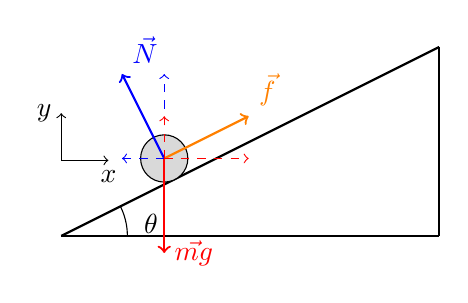
\begin{tikzpicture}[scale=1.2]
  \draw[thick] (0,0) -- (4,0);
  \draw[thick] (0,0) -- (4,2);
  \draw[thick] (4,0) -- (4,2);
  \filldraw[fill=gray!30] (1.09,0.82) circle (0.25);
  \draw[->,thick,red] (1.09,0.82) -- ++(0,-1) node[right] {$\vec{mg}$};
  \draw[->,thick,blue] (1.09,0.82) -- ++(-0.447,0.894) node[above right] {$\vec{N}$};
  \draw[->,thick,orange] (1.09,0.82) -- ++(0.894,0.447) node[above right] {$\vec{f}$};
  \draw[->] (0,0.8) -- ++(0,0.5) node[left] {$y$};
  \draw[->] (0,0.8) -- ++(0.5,0) node[below] {$x$};
  \draw[->,dashed, blue] (1.09,0.82) -- ++(0,0.894) node[left] {};
  \draw[->,dashed, blue] (1.09,0.82) -- ++(-0.447,0) node[below] {};
  \draw[->,dashed, red] (1.09,0.82) -- ++(0.894,0) node[below right] {};
  \draw[->,dashed, red] (1.09,0.82) -- ++(0,0.447) node[left] {};
  \draw (0.7,0) arc (0:26.565:0.7);
  \node at (0.95,0.13) {$\theta$};
\end{tikzpicture}\\
沿斜面和垂直斜面分解
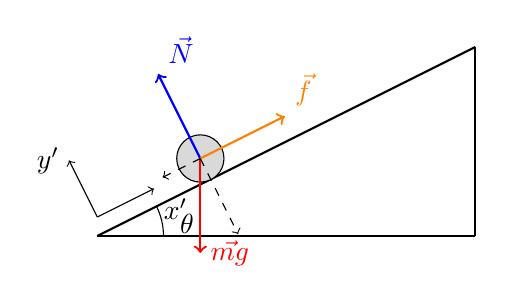
\begin{tikzpicture}[scale=1.2]
  \draw[thick] (0,0) -- (4,0);
  \draw[thick] (0,0) -- (4,2);
  \draw[thick] (4,0) -- (4,2);
  \filldraw[fill=gray!30] (1.09,0.82) circle (0.25);
  \draw[->,thick,red] (1.09,0.82) -- ++(0,-1) node[right] {$\vec{mg}$};
  \draw[->,thick,blue] (1.09,0.82) -- ++(-0.447,0.894) node[above right] {$\vec{N}$};
  \draw[->,thick,orange] (1.09,0.82) -- ++(0.894,0.447) node[above right] {$\vec{f}$};
  \draw[->,dashed] (1.09,0.82) -- ++(-0.4,-0.2) node[above right] {};
  \draw[->,dashed] (1.09,0.82) -- ++(0.4,-0.8) node[left] {};
  \draw[->] (0,0.2) -- ++(0.6,0.3) node[below right] {$x'$};
  \draw[->] (0,0.2) -- ++(-0.3,0.6) node[left] {$y'$};
  \draw (0.7,0) arc (0:26.565:0.7);
  \node at (0.95,0.13) {$\theta$};
\end{tikzpicture}\\
物理中最常见的三角形：
\begin{tikzpicture}[scale=1.2]
  \coordinate (A) at (0,0);
  \coordinate (B) at (4,0);
  \coordinate (C) at (4,3);
  \draw[thick] (A) -- (B) -- (C) -- cycle;
  \node[below] at ($(A)!0.5!(B)$) {4};
  \node[right] at ($(B)!0.5!(C)$) {3};
  \node[above left] at ($(A)!0.5!(C)$) {5};
  \draw (A) ++(0.5,0) arc (0:37:0.5);
  \node at (0.7,0.18) {$37^\circ$};
  \node[left] at (A) {A};
  \node[below right] at (B) {B};
  \node[above right] at (C) {C};
\end{tikzpicture}
}
\newpage
 \section{共点力平衡}
\concept{受力分析怎么做？}{重力先画，不一定要画在重心位置，或者是中心点，挑一个好看的地点更好，比如图中已经有很多直线了，选择那些直线的交点。这样可以让图像更清晰。
弹力是一个难点，牢记我们之前的规律应用他们，
最后再画摩擦力，因为有弹力才能有摩擦力。
总结为1重2弹3摩擦。最后题目中还有别的外力再补充。
二力平衡，一定是等大反向，作用于同一个物体。，方向是一条直线上。
不共线的三力平衡一定是形成一个首尾相连的密闭三角形。
多个力作用平衡时，任意一个力与其他力的合力是二力平衡。
在上面的过程中，唯一需要注意的就是，多个力的合力不要和其他任何一个分力同时存在，一旦选择了合成，那么这些力就应该消失。
正交分解处理平衡问题，只需要在两个垂直的方向上，合力为0就是平衡。一个方向平衡，那么就是那个方向上合力为0.
总结一下：三个力及以上，我们很少使用正交分解方法，最多使用正弦定理。四个力则基本上都要用正交分解解决。}
\newpage
\section{受力分析综合提升专题}
\concept{弹力、摩擦力判断有无}{假设法，假设不存在或者假设存在，判断能够保持平衡，如果可以那么假设正确，如果无法，那么假设错误。同样的先假设弹力再假设摩擦力，因为先有弹力才有摩擦力。
弹簧弹力的计算，和伸长量成正比，一定要记住，弹簧有一个位置是原长位置。这个位置相当重要，大家在后面选修和牛顿运动定律都会有弹簧，这个万恶的东西，比较难。
摩擦力，里面的计算一定要注意，静摩擦力是大小未知的，和平衡状态有关，最大静摩擦力和正压力相关，一般而言题目会假定最大静摩擦力等于滑动摩擦力，但是不是一定的，一定一定要注意这个问题，但是有的时候题目确实说法不够严谨的，尤其是校级考试，那没办法，就认为这件事情是默认的。}
\newpage
\section{牛顿运动定律}
\concept{伽利略理想斜面实验}{三个实验推断过程}
\concept{牛顿第一运动定律（惯性定律）}{质量是惯性的量度，质量越大惯性就越大。
惯性是物体改变运动状态难易程度的体现
为什么我们之前质点，保留了质量呢？就是因为质量会影响惯性，而惯性会影响物体运动状态改变。所以运动学问题需要质量。}
\equations{
    F_{12}=-F_{21}
}
\concept{牛顿第三运动定律（相互作用力）}{作用力与反作用力大小相等，作用物体和施加物体不同，方向相反，作用于不同物体。}
\equations{
    F_\text{合}=ma
}
\concept{牛顿第二运动定律（非常非常重要的定律）}{成功将运动学和力学变成了一个统一的学科，力学，因为运动就是力的反应。力可以影响运动。
F=ma里面的加速度是瞬时加速度，这就是我们以前提到过的，这才是加速度的定义式，能够决定任意时刻的加速度，并且只要物体的力改变了，物体的加速度就会改变。
不同方向的力能得到对应方向的加速度。
并且我们之前的受力平衡，其实你会发现牛二里面如果加速度是0，就是平衡问题。
对于之前我们的正交分解由此多了一种分解方法，沿加速度和垂直加速度分解，这样就不用分解加速度。
}
\concept{国际单位制，（量纲法）}{你知道吗？这可是一个高考考点，简单来说就是单位可以计算。
做选择题至此大家已经收获了一个强大的方法，量纲法，选择题做之前先用量纲法试一试。
这些单位里面记一下基本物理量就行，比如力学就是长度和时间与质量，电学需要电流就行，这个能够定义电场和磁场。热学需要物质的量和温度，压强用力学就行，光学里面加上一个发光强度。}
\end{document}